\begin{frame}{Xác thực đa yếu tố bằng thuật toán TOTP}
\begin{figure}[H]
\centering
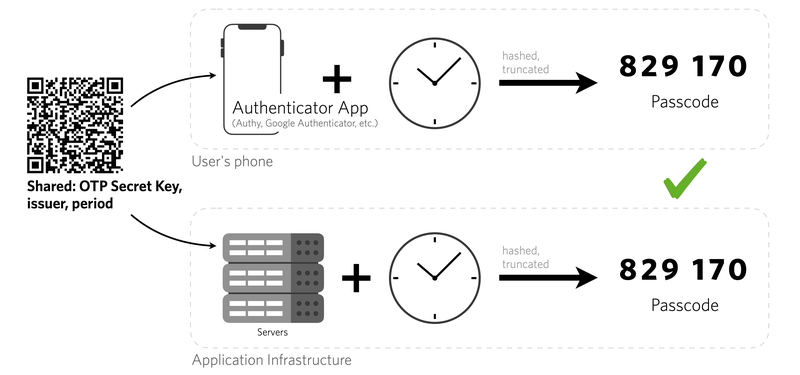
\includegraphics[height=0.55\textheight,width=0.9\textwidth,keepaspectratio]{pictures/2fa_diagram.jpg}

\caption[Cách hoạt động của TOTP]{Cách hoạt động của TOTP (Nguồn: \footnotemark)}
\end{figure}
\footnotetext{\url{https://www.twilio.com/en-us/blog/developers/tutorials/product/authy-api-and-google-authenticator}}

\note{
Để tăng cường bảo mật cho tài khoản, hệ thống hỗ trợ xác thực đa yếu tố (MFA) bằng thuật toán TOTP (Time-based One-time Password).
Mã khóa bí mật được máy chủ tạo ra và hiển thị dưới dạng mã QR. Người dùng dùng ứng dụng Authenticator để quét và lưu trữ. Mỗi 30 giây, ứng dụng và máy chủ sẽ tự động tính toán ra một mã số gồm 6 chữ số dựa trên thời gian thực. Khi đăng nhập, người dùng nhập mã này để đối chiếu.
}
\end{frame}
